\chapter{Zielsetzung}\label{ch:zielsetzung}
Eine effiziente Ressourcennutzung ist für Unternehmen von zentraler Bedeutung. Produktionsprobleme können dabei enorme finanzielle
Verluste verursachen, wie das Beispiel von Volkswagen im Jahr 2016 zeigt: Durch Störungen im Fertigungsprozess entstand ein wöchentlicher
Schaden von bis zu 400 Millionen Euro~\cite{Krupitzer2020}. Zudem zeigen Studien, dass je nach Branche zwischen 15 und 70~\% der
Produktionskosten auf wartungstechnische Ursachen zurückzuführen sind~\cite{Bevilacqua2000}.

Jedoch liegt der Fokus dieser Arbeit nicht auf wirtschaftlichen Faktoren. Trotzdem ist zu erwähnen, dass neue, effiziente
Wartungsstrategien basierend auf der Überwachung wichtiger Systemparameter insgesamt eine wirtschaftlichere und kostengünstigere
Alternative zu klassischen Wartungsstrategien (vgl.~\hyperref[sec:trad_maintenance]{Abs.~\Ref*{sec:trad_maintenance}})
darstellen~\cite{Deloux2009}~\Cite[S.~64--65]{Mobley2002}.

Der Fokus liegt vielmehr in der Entwicklung, Erprobung und Umsetzung der zugrundeliegenden technischen Fragestellung: \textbf{Wie können
Unsupervised Learning Algorithmen zur Anomaliedetektion genutzt werden, um zur Entwicklung eines effizienten Wartungssystems
beizutragen?}

\begin{figure}[H]
    \centering
    \begin{tikzpicture}
        \node[anchor=south west,inner sep=0] (image) at (0,0) {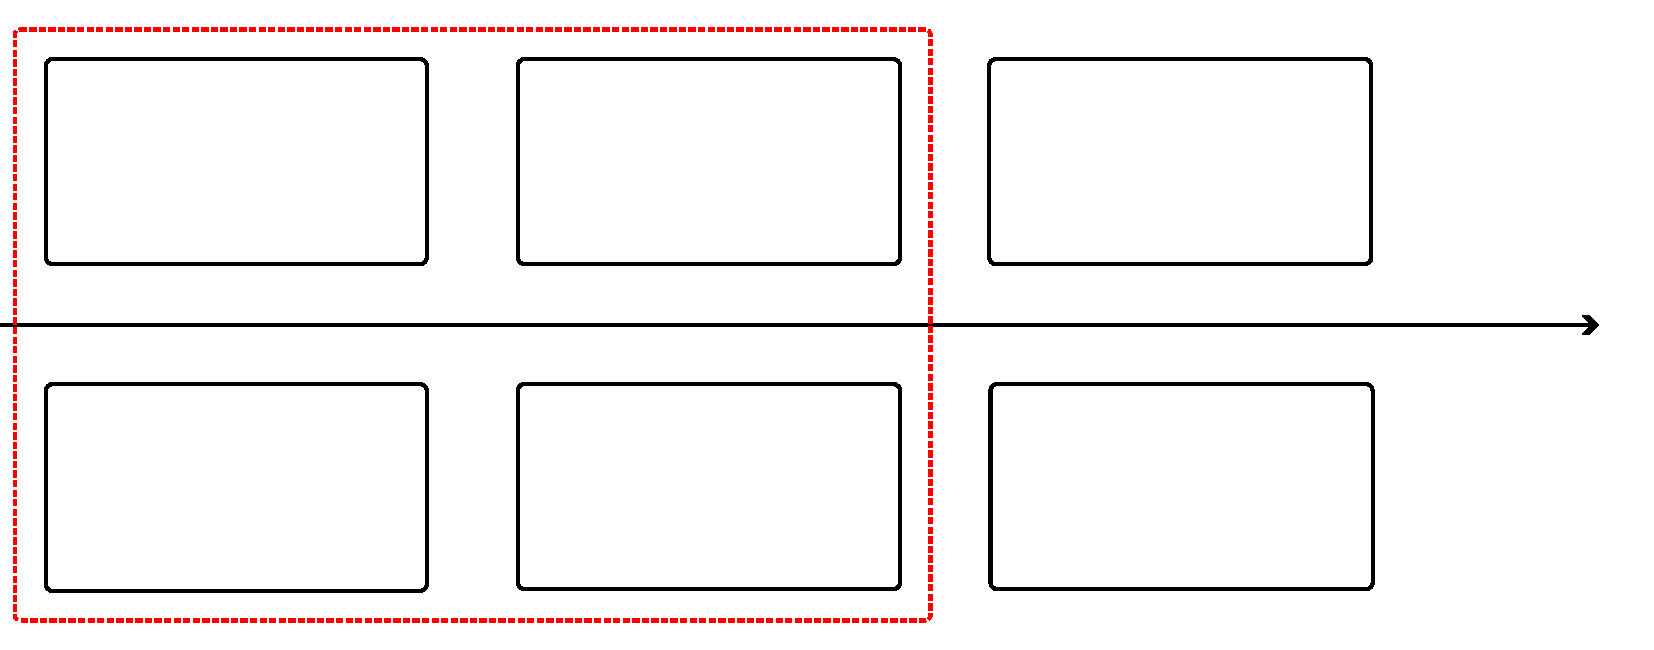
\includegraphics[width=\linewidth]{ch2_zielsetzung/abbildungen/zielsetzung_scope.pdf}};
        % Koordinatensystem für die Grafik
        \begin{scope}[x={(image.south east)},y={(image.north west)}]
            % Textpositionen anpassen:
            \node at (0.145,0.74) {\large\parbox{6cm}{\centering Daten-\\aggregierung}};
            \node at (0.145,0.26) {\large\parbox{6cm}{\centering Recherche\\sich eignender\\Algorithmen}};
            \node at (0.43,0.74) {\large\parbox{4cm}{\centering Implementierung \&\\Erprobung der\\Algorithmen}};
            \node at (0.43,0.26) {\large\centering Evaluierung};
            \node at (0.715,0.74) {\large\parbox{4cm}{\centering Ableitung\\geeigneter\\Maßnahmen}};
            \node at (0.715,0.26) {\large\parbox{4cm}{\centering Schulen und Finden\\geeigneter\\Mitarbeiter}};
            \node at (0.85,0.46) {\centering Entwicklungsfortschritt};
            \node at (0.2875,0) {\centering \textcolor{red}{\large\textbf{Fokus der Arbeit}}};
            \node at (0.9,0.74) {\centering \dots};
            \node at (0.9,0.26) {\centering \dots};
        \end{scope}
    \end{tikzpicture}
    \caption{Entwicklungsprozess eines auf Predictive Maintenance basierenden Wartungssystems}
~\label{fig:zielsetzung_scope}
\end{figure}

Alle weiteren, impliziten Konsequenzen, wie eine Reduzierung der Downtime, Verbesserung der Systemzuverlässigkeit
und Gerätelaufzeit, eine Verbesserung der Produktqualität oder die Redundanz eines großen
Ersatzteillagers~\cite[S.~61--62]{Mobley2002}~\Cite[S.~5]{Scheffer2004} wollen im Rahmen dieser Arbeit nicht betrachtet werden.

Die starke Eingrenzung der Zielsetzung erfolgt auch aufgrund des gegebenen zeitlichen Rahmens der Arbeit von zehn Wochen. Das primäre
Ziel ist also vielmehr die Erprobung verschiedener, sich als potenziell geeignet heraustellender, Machine Learning Algorithmen zur
Anomaliedetektion. Dabei gibt es aufgrund der sich zum Teil sehr grundlegend unterscheidenden Arten von Anomalien entsprechend pro
Anomalietyp separate Kandidaten. Die voneinander abweichenden Anomaliearten und die dafür jeweils nominierten Algorithmen werden in
\hyperref[ch:anomaliedetektion]{Kap.~\Ref*{ch:anomaliedetektion}} vorgestellt und erläutert.

Die Erprobung der einzelnen Algorithmen erfolgt anhand der Anomalietypen, denen sie am besten zugeordnet werden können. Doch in
Studien zeigt sich, dass einzelne Algorithmen auch interdisziplinär, also für mehrere, sehr unterschiedliche Anomalietypen, gut
abschneiden~\cite[S.~30~-~31]{Wenig2024}\cite{Schmidl2022}. Daher sollen alle Algorithmen auch überschneidend getestet werden, um ein ganzheitliches Bild zu erhalten.
Der Kontext der Arbeit soll an dieser Stelle noch einmal hervorgehoben werden. Für industrielle Zwecke ist es vorteilhafter, sich auf eine
weniger umfangreiche Lösung zu konzentrieren, mit der aber mehrere Fehlerfälle abgedeckt oder vorhergesagt werden können, statt einzelne,
hochspezialisierte Lösungen zu finden. Die Robustheit eines Algorithmus ist daher genauso wichtig wie die Fähigkeit, jede Anomalie bis
ins letzte Detail zu erkennen. Auch diese Einordnung soll in der Findung der optimalen Lösung berücksichtigt werden.

Zur Bewertung und Einordnung der Ergebnisse der Algorithmen ist auch eine Evaluierungsmethode notwendig. Allerdings soll diese nicht
vollautomatisiert sein, sondern nach dem sog.~\textit{Human-in-the-Loop} Ansatz geschehen. So kann die Expertise geschulter und
erfahrener Mitarbeitenden in die Evaluierung miteingebunden werden, zur besseren Beurteilung und Korrektur der Ergebnisse~\cite{Deng2024}.

Schlussendlich und ausblickend soll diese Arbeit einen Beitrag zu besser getimten Wartungseinsätzen beitragen~-~nicht nur für die SSPX1,
sondern für weitere Systeme der Vitronic Produktfamilie, da die zu Grunde liegenden, analysierten Parameter nicht exklusiv zur SSPX1 gehören.